\chapter{Theoretical Background} % <<< --------------------------------------- %
\label{ch:analog-to-digital_data_aquisition}
% ---------------------------------------------------------------------------- %

This chapter  will present a  brief synopsis on  some aspects of  digital data
acquisition from  an analog source  and the processing  of that data,  and how
those issues pertain to our project. It  is not intended to be a comprehensive
treatise on the subject but shall serve  as a short refresher. At its end, the
reader should  have sufficient insight  to understand the basic  motivation of
our project from a theoretical point of view.

TODO: references to more comprehensive literature.

\section{The Digital Signal Processing Chain}% <<< --------------------------- %
\label{sec:dsp_chain}

Digitally acquiring a signal generally requires at least the following steps:
\begin{itemize}\tightlist
        \item
            Passing the signal through an analog low-pass filter.
        \item
            Sampling and quantizing the filtered signal.
\end{itemize}

The   resulting   sequence  of   values   can   then  be   further   digitally
processed. The necessary  building blocks  for this  process are  portrayed in
Figure~\ref{fig:dspChain:blocks}.

\begin{figure}
    \centering
    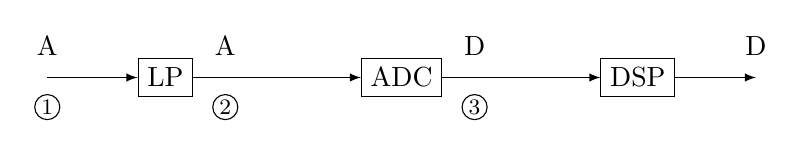
\begin{tikzpicture}
    \coordinate (in) at (-1.5,0);
    \coordinate (out) at (7.5,0);

    \node[draw] (LP)  at (0,0) {LP};
    \node[draw] (ADC) at (3,0) {ADC};
    \node[draw] (DSP) at (6,0) {DSP};

    \draw[-latex] (in)  -- (LP);
    \draw[-latex] (LP)  -- (ADC);
    \draw[-latex] (ADC) -- (DSP);
    \draw[-latex] (DSP) -- (out);

    \node[above      =1ex] (a1a) at (in)       {A};
    \node[above right=1ex] (a2a) at (LP.east)  {A};
    \node[above right=1ex] (d1a) at (ADC.east) {D};
    \node[above      =1ex] (d2a) at (out)      {D};

    \node[draw,circle,below=4ex,inner sep=0.30mm] (a1b) at (a1a) {\footnotesize 1};
    \node[draw,circle,below=4ex,inner sep=0.30mm] (a2b) at (a2a) {\footnotesize 2};
    \node[draw,circle,below=4ex,inner sep=0.30mm] (d1b) at (d1a) {\footnotesize 3};
\end{tikzpicture}

    \caption{%
        The basic  building blocks of the  DSP chain from its  analog input to
        its digitally processed output.\protect\newline
        From  left  to  right: The  analog low-pass  filter  (\emph{LP}),  the
        analog-to-digital  converter (\emph{ADC}),  and  an arbitrary  digital
        signal processing  system for further  processing of the  ADC's output
        (\emph{DSP}).%
    }
    \label{fig:dspChain:blocks}
\end{figure}

\begin{figure}
    \centering
    \begin{tikzpicture}
     \pgfplotsset{every axis/.style={
            height=30mm,
            width=40mm,
            grid=none,
            axis line style={draw=none},
            tick style={draw=none},
            ticks = none,
        }
    }
    \begin{axis}[
        at = {(0,0)},
    ]
        \addplot[-]            table[x=t,y=y,col sep=comma] {images/dspChain/noisySine.csv};
    \end{axis}

    \begin{axis}[
        at = {(40mm,0)},
    ]
        \addplot[-,smooth]     table[x=t,y=y,col sep=comma] {images/dspChain/smoothSine.csv};
    \end{axis}

    \begin{axis}[
        at = {(80mm,0)},
    ]
        \addplot[ycomb,mark=o,mark size=1.0] table[x=t,y=y,col sep=comma] {images/dspChain/sampledSine.csv};
    \end{axis}
    \draw[-latex] (2.5,0.75) -- (3.85,0.75);
    \draw[-latex] (6.5,0.75) -- (7.85,0.75);

    \node[draw,inner sep=0.3mm,circle] at (1.25,1.75) {\footnotesize 1};
    \node[draw,inner sep=0.3mm,circle] at (5.25,1.75) {\footnotesize 2};
    \node[draw,inner sep=0.3mm,circle] at (9.25,1.75) {\footnotesize 3};
\end{tikzpicture}

    \tikzsetnextfilename{dspChainFreqDomain}
\begin{tikzpicture}
     \pgfplotsset{every axis/.style={
            height=25mm,
            width=30mm,
            grid=none,
            axis line style={draw=none},
            tick style={draw=none},
            ticks = none,
        }
    }
    \begin{axis}[
        at = {(0,0)},
    ]
        \addplot[thick,q1,-]
            table[x=t,y=y,col sep=comma] {images/dspChain/spectrumFlat.csv};
    \end{axis}

    \begin{axis}[
        at = {(40mm,0)},
    ]
        \addplot[thick,q1,-,smooth]
            table[x=t,y=y,col sep=comma] {images/dspChain/spectrumLP.csv};
    \end{axis}

    \begin{axis}[
        at = {(80mm,0)},
    ]
        \addplot[thick,q1,-,smooth]
            table[x=t,y=y,col sep=comma] {images/dspChain/spectrumSampled.csv};
    \end{axis}
    \draw[-latex] (2.9,1.25) -- (3.95,1.25);
    \draw[-latex] (6.9,1.25) -- (7.95,1.25);

    %\node[draw,inner sep=0.3mm,circle] at (1.25,1.75) {\footnotesize 1};
    %\node[draw,inner sep=0.3mm,circle] at (5.25,1.75) {\footnotesize 2};
    %\node[draw,inner sep=0.3mm,circle] at (9.25,1.75) {\footnotesize 3};
\end{tikzpicture}

    \caption{%
        Simplified  time-domain  (top)   and  frequency-domain  (bottom)  view
        of  the  signal  at  different  stages on  its  way  through  the  DSP
        chain. The circled  numbers correspond  to the  stages as  outlined in
        Figure~\ref{fig:dspChain:blocks}.\protect\newline
        Stage  1 is  the  signal  before passing  through  the input  low-pass
        filter,  with  a  significant   amount  of  high-frequency  noise. The
        low-pass filter removes any  frequency components above ${f_s}/{2}$ in
        an ideal scenario  (in reality, it merely attenuates them,  as we will
        see later), resulting in the signal at stage 2.\protect\newline
        After having been filtered, the  ADC samples and quantizes the signal,
        yielding  a sequence  of  values, as  schematically  portrayed in  the
        rightmost picture for stage 3.\protect\newline
        Note that  due to the sampling  process, the spectrum of  the filtered
        signal is repeated at intervals of  $f_s/2$. This is the source of the
        issue of \emph{aliasing}.%
    }
    \label{fig:dspChain:signals}
\end{figure}

Of particular  interest for our  application is  what happens in  the ADC. The
quantization process converts a  value-continuous signal into a value-discreet
one,  with its  resolution being  a specification  of the  ADC which  is being
used. As an example, the ADC in our system has a resolution of \num{14}\,bits,
meaning it can divite its valid  input range into \num{16384} values. Given an
input range of \SI{2}{\volt} $V_{PP}$, that equates to a resolution of roughly
\SI{122}{\micro\volt} (in theory). This quantization  process is the source of
what is generally  known as \emph{quantization noise}. For more  on the topic,
see \code{TODO}.

TODO: Check numbers. Give references for further reading.

Besides the quantization,  the other step happening in the  ADC is sampling; a
time-continuous signal is converted into a series of time-discreet values. The
time between those values is known as \emph{sampling time}, its inverse is the
\emph{sampling  frequency}. Note that  usually  these are  constant, at  least
during the  time where the signal  is measured. This need not  strictly be the
case  in theory  though. In our  system, this  sampling frequency  is a  fixed
property of the ADC, and is \SI{125}{\mega\hertz}.

The sampling  step lies  at the  core of  the problem  our project  intends to
address:  \emph{aliasing}. Therefore, we  will take  a  closer look  at a  few
consequences  of the  sampling  process, and  how they  are  relevant to  this
project.

Descriptively, the sampling  process can be thought of as  looking at a signal
at  specific points  in  time and  capturing  its value. Mathematically,  this
amounts to multipliying the  signal with a series of Dirac  pulses in the time
domain,  and  convolving with  a  series  of  Dirac  pulses in  the  frequency
domain\footnotemark.
\footnotetext{%
    \emph{Pro memoria}: A series of Dirac pulses  in the time domain has as its
    spectrum a series of Dirac pulses as well.%
}.
This  convolution  in   the  frequency  domain  lies  at  the   heart  of  the
problem   of  aliasing,   because  it   results  in   the  incoming   signal's
spectrum  being  repeated  at  intervals  of  $f_s$  (see  also:  stage  3  in
Figure~\ref{fig:dspChain:signals}). This is no problem as long as the spectrum
of the incoming signal fits within  the boundaries set by this repetition. But
if  the  spectrum   of  the  incoming  singal  is  too   broad,  two  or  more
recurrences  of  the spectrum  will  overlap. This  effect is  highlighted  in
Figure~\ref{fig:aliasing:band}.

\begin{figure}
    \centering
    \begin{tikzpicture}
     \pgfplotsset{every axis/.style={
            height=40mm,
            width=120mm,
            grid=none,
            axis line style={draw=none},
            tick style={draw=none},
            ticks = none,
        }
    }
    \begin{axis}[
        at = {(0mm,30mm)},
    ]
        \addplot[-]            table[x=f,y=Y,col sep=comma] {images/aliasing/bandNoAliasing.csv};
    \end{axis}

    \begin{axis}[
        at = {(0mm,0mm)},
    ]
        \addplot[-]            table[x=f,y=Y,col sep=comma] {images/aliasing/bandAliased1.csv};
        \addplot[-]            table[x=f,y=Y,col sep=comma] {images/aliasing/bandAliased2.csv};
        \addplot[-]            table[x=f,y=Y,col sep=comma] {images/aliasing/bandAliased3.csv};
    \end{axis}
\end{tikzpicture}

    \caption{%
        Simplified view  of a signal  which does not produce  aliasing between
        its recurrences  in the  frequency spectrum  (top), contrasted  with a
        signal whose  frequency band  has components  above half  the sampling
        frequency,  resulting   in  aliasing;  its  spectral   copies  overlap
        (highlighted areas in the bottom plot).%
    }
    \label{fig:aliasing:band}
\end{figure}

This overlap results in two primary problems:
\begin{itemize}\tightlist
    \item
        The digital  signal may not  be unambiguously reconstructable  into an
        analog signal, if that is intended.
    \item
        Frequencies  may occur  in the  digital  signal stream  which are  not
        actually  present  in  the  original  signal. This  problem  is  often
        referred to  as the  \emph{folding back} of  frequency components. See
        Figure~\ref{fig:aliasing:dirac} for an illustration  of how this might
        look.

        This problem is of particular interest  to our application, as we will
        see later.
\end{itemize}

\begin{figure}
    \centering
    \begin{tikzpicture}
     \pgfplotsset{every axis/.style={
            height=40mm,
            width=120mm,
            grid=none,
            axis line style={draw=none},
            tick style={draw=none},
            ticks = none,
        }
    }
    % fs = 4
    % fs/2 = 2
    
    % Dirac at f=1
    \begin{axis}[
        at = {(0mm,30mm)},
    ]
        % Centered around 0
        \addplot[ycomb,mark=triangle*] coordinates {
            (1,1)
            (-1,1)
        };
        % Centered around fs = 4
        \addplot[blue,ycomb,mark=triangle*] coordinates {
            (3,1)
            (5,1)
        };
        % Centered around -fs = -4
        \addplot[magenta,ycomb,mark=triangle*] coordinates {
            (-3,1)
            (-5,1)
        };
    \end{axis}

    % Dirac at f=3
    \begin{axis}[
        at = {(0mm,0mm)},
    ]
        % Centered around 0
        \addplot[ycomb,mark=triangle*] coordinates {
            (3,1)
            (-3,1)
        };
        % Centered around fs = 4
        \addplot[blue,ycomb,mark=triangle*] coordinates {
            (1,1)
            (7,1)
        };
        % Centered around -fs = -4
        \addplot[magenta,ycomb,mark=triangle*] coordinates {
            (-1,1)
            (-7,1)
        };
    \end{axis}
\end{tikzpicture}

    \caption{%
        Example  of  two harmonic  signals  being  sampled. In the  top  plot,
        the  signal's  frequency is  below  half  the sampling  frequency  and
        there  is  no  aliasing. The   signal  can  be  reconstructed  without
        error.\protect\newline
        In the bottom plot, the signal's  frequency is above half the sampling
        frequency. Consequently, the copies of the signal's frequency spectrum
        centered around  the sampling  frequency and  its negative  alias back
        into  the  band  between  $-f_s/2$  and  $f_s/2$. If  this  signal  is
        reconstructed, the resulting  signal would have a frequency  of $f_s -
        f_{\mathrm{sig}}$ instead of $f_{\mathrm{sig}}$.%
    }
    \label{fig:aliasing:dirac}
\end{figure}


Once a signal  has left the ADC and  is handed down the DSP  chain for further
processing,  the primary  problem becomes  one of  resources, particularly  in
real-time applications. In  most systems,  the available  hardware is  a fixed
constraint, and depending on what sort of processing is to be conducted on the
digital data stream, the available resources may or may not suffice.

If available resources are found to be insufficient for real-time processing of
the data stream, one may choose to
\begin{itemize}\tightlist
    \item
        not process the data in real time,
    \item
        reduce the complexity of the computations, or
    \item
        reduce the amount of data to be processed through \emph{downsampling}
        of the signal.
\end{itemize}
The  last case  is the  route  which is  chosen in  our application. The  main
constraint on the Red Pitaya is that  the data being generated cannot be moved
off the  device in  real time,  and the  device itself  does not  really offer
sufficient storage for capturing a meaningful amount of data which can then be
moved onto another  device for further processing at  a later point. Therefore
the amount of data must be reduced before  it can be moved off the device to a
computer for viewing or further processing.

TODO: Amount of data being generated on the PITA.

Because downsampling a signal is in  essence nothing more than the sampling of
a signal which has already been sampled, a lot of the considerations which are
valid for the  step from an analog  to a digital signal as  outlined above are
either very  similar or even identical. Specifically,  the same considerations
for  aliasing still  apply: If  the  signal which  is  to  be downsampled  has
frequency components  above $f_{s,  downsampled}/2$, aliasing  will occur. And
since the  signal coming out of  the ADC has the  original signal's (filtered)
spectrum recurring at intervals of its  sampling frequency, this is always the
case.\code{TODO: Correct?}

Therefore,  the sampled  signal must  be  filtered through  a low-pass  filter
before  being downsampled,  just as  the original  analog signal  was low-pass
filtered  before being  passed into  the  ADC. In light  of the  signal to  be
downsampled  being a  \emph{digital} signal  instead  of an  analog one,  that
low-pass filter must  naturally be a digital filter as  well. Designing such a
digital low-pass filter is the core mission of this project.


%\subsection{Challenges in Downsampling}
%\label{subsec:downsampling}
%
%The most obvious way to downsample from a sequence of values is of course to simply pick
%each nth sample. However, this has some serious drawbacks which make it an unworkable solution
%in most cases.
%
%\textbf{Fancy Graphics of downsampling without LP filter with explanations}
%
%
%\subsection{Digital Low-Pass Filters}
%\label{subsec:digital-lp-filters}
%
%The obvious solution to this predicament is to apply a (digital) low-pass filter to the
%sequence of values before downsampling. For this purpose, three types of filters are commonly
%used, each with their own specific advantages and drawbacks: IIR, FIR, CIC.
%
%For theseandthose reasons, we will use FIR and CIC in our system.
%
%\textbf{Fancy graphics of LP filter, downsampling and folding back}
%
%%>>>
%
%\section{Designing a Filter System}
%\label{sec:designing-a-filter-system}
%
%Talking about which type of filter has which properties is all good and well in theory, but
%how does one actually apply this knowledge to a practical problem? This section answers that
%question insofar as it applies to our project.
%
%\begin{itemize}\tightlist
%    \item
%        limited HW resources
%    \item
%        single-stage vs. multi-stage
%    \item
%        TBW issue with multi-stage
%    \item
%        filters at lower frequencies use fewer resources
%    \item
%        halfband filtres
%    \item
%        CIC: compensation filters
%\end{itemize}
\clearpage
\begin{figure}
    \centering
    \tikzsetnextfilename{firTopology}
% https://tex.stackexchange.com/a/183092/131649
\begin{tikzpicture}[
    triangle/.style = {draw,regular polygon, regular polygon sides=3 },
    node rotated/.style = {rotate=180},
    border rotated/.style = {shape border rotate=180}
]    
    \coordinate (in) at   (0,0);
    \coordinate (out) at (12,-2);

    % Delay elements
    \node[draw] (d1) at  (2,0) {$z^{-1}$};
    \node[draw] (d2) at  (4,0) {$z^{-1}$};
    \node[draw] (d3) at  (6,0) {$z^{-1}$};
    \node       (d4) at  (8,0) {\ldots};
    \node[draw] (d5) at (10,0) {$z^{-1}$};

    % Multipliers
    \node[triangle, border rotated] (m1) at  (1,-1) {};
    \node[triangle, border rotated] (m2) at  (3,-1) {};
    \node[triangle, border rotated] (m3) at  (5,-1) {};
    \node[triangle, border rotated] (m4) at  (7,-1) {};
    \node[triangle, border rotated] (m5) at (11,-1) {};

    % Adders
    \node[draw,circle, inner sep=0.3mm] (a1) at  (3,-2) {$+$};
    \node[draw,circle, inner sep=0.3mm] (a2) at  (5,-2) {$+$};
    \node[draw,circle, inner sep=0.3mm] (a3) at  (7,-2) {$+$};
    \node                               (a4) at  (9,-2) {\ldots};
    \node[draw,circle, inner sep=0.3mm] (a5) at (11,-2) {$+$};

    % Lines
    \draw[-latex] (in) -- (d1);
    \draw[-latex] (in) -| (m1);
    \draw[-latex] (d1) -- (d2);
    \draw[-latex] (d1) -| (m2);
    \draw[-latex] (d2) -- (d3);
    \draw[-latex] (d2) -| (m3);
    \draw[-latex] (d3) -- (d4);
    \draw[-latex] (d3) -| (m4);
    \draw[-latex] (d4) -- (d5);
    \draw[-latex] (d5) -| (m5);
    \draw[-latex] (m1) |- (a1);
    \draw[-latex] (m2) -- (a1);
    \draw[-latex] (a1) -- (a2);
    \draw[-latex] (m3) -- (a2);
    \draw[-latex] (a2) -- (a3);
    \draw[-latex] (m4) -- (a3);
    \draw[-latex] (a3) -- (a4);
    \draw[-latex] (a4) -- (a5);
    \draw[-latex] (m5) -- (a5);
    \draw[-latex] (a5) -- (out);
\end{tikzpicture}

    \caption{Digital signal processing chain from analog signal to the digitally processed data stream}
    \label{fig:filtertopologies:fir}
\end{figure}

\begin{figure}
    \centering
    \tikzsetnextfilename{iirTopology}
% https://tex.stackexchange.com/a/183092/131649
\begin{tikzpicture}[
    triangle/.style = {draw,regular polygon, regular polygon sides=3 },
    node rotated/.style   = {rotate=180},
    border rotatedA/.style = {shape border rotate=-90},
    border rotatedB/.style = {shape border rotate=90},
]    
    \coordinate (in)  at (0,0);
    \coordinate (out) at (8,0);

    % Delay elements
    \node[draw] (d1) at  (2,-1) {$z^{-1}$};
    \node[draw] (d2) at  (2,-3) {$z^{-1}$};
    \node[draw] (d3) at  (6,-1) {$z^{-1}$};
    \node[draw] (d4) at  (6,-3) {$z^{-1}$};

    % Multipliers
    \node[triangle, border rotatedA] (m1) at  (3,0) {};
    \node[triangle, border rotatedA] (m2) at  (3,-2) {};
    \node[triangle, border rotatedA] (m3) at  (3,-4) {};
    \node[triangle, border rotatedA] (m4) at  (5,0) {};
    \node[triangle, border rotatedB] (m5) at  (5,-2) {};
    \node[triangle, border rotatedB] (m6) at  (5,-4) {};

    %% Adders
    \node[draw,circle, inner sep=0.3mm] (a1) at  (4,0) {$+$};
    \node[draw,circle, inner sep=0.3mm] (a2) at  (4,-2) {$+$};
    \node[draw,circle, inner sep=0.3mm] (a3) at  (4,-4) {$+$};

    %% Lines
    \draw[-latex] (in) -- (m1);
    \draw[-latex] (in) -| (d1);
    \draw[-latex] (d1) -- (d2);
    \draw[-latex] (d1) |- (m2);
    \draw[-latex] (d2) |- (m3);
    \draw[-latex] (m1) -- (a1);
    \draw[-latex] (m2) -- (a2);
    \draw[-latex] (m3) -- (a3);
    \draw[-latex] (a1) -- (m4);
    \draw[-latex] (m5) -- (a2);
    \draw[-latex] (m6) -- (a3);
    \draw[-latex] (d3) |- (m5);
    \draw[-latex] (d3) -- (d4);
    \draw[-latex] (d4) |- (m6);
    \draw[-latex] (m4) -| (d3);
    \draw[-latex] (m4) -- (out);
\end{tikzpicture}

    \caption{Digital signal processing chain from analog signal to the digitally processed data stream}
    \label{fig:filtertopologies:iir}
\end{figure}

\begin{figure}
    \centering
    %\tikzsetnextfilename{cicTopology}
% https://tex.stackexchange.com/a/183092/131649
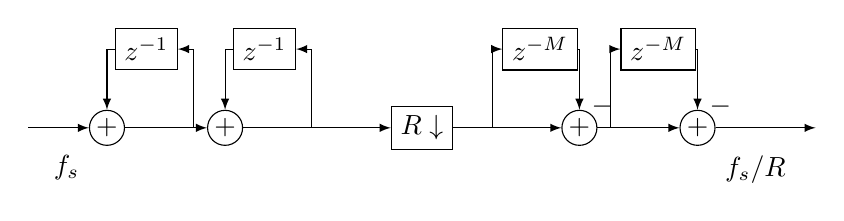
\begin{tikzpicture}
    \coordinate (in)  at  (0,0);
    \coordinate (out) at (10,0);

    % branching coordinates
    \coordinate (b1) at (2.1,0); % delta: 1.5
    \coordinate (b2) at (3.6,0); % delta: 1.5
    \coordinate (b3) at (5.9,0); % delta: 1.8
    \coordinate (b4) at (7.4,0); % delta: 1.5

    % Delay elements
    \node[draw] (d1) at  (1.5,1) {$z^{-1}$};
    \node[draw] (d2) at  (3.0,1) {$z^{-1}$};
    \node[draw] (d3) at  (6.5,1) {$z^{-M}$};
    \node[draw] (d4) at  (8.0,1) {$z^{-M}$};

    % Downsampler
    \node[draw] (r1) at (5,0) {$R\downarrow$};

    % Adders
    \node[draw,circle, inner sep=0.3mm] (a1) at  (1.0,0) {$+$};
    \node[draw,circle, inner sep=0.3mm] (a2) at  (2.5,0) {$+$};
    \node[draw,circle, inner sep=0.3mm] (a3) at  (7.0,0) {$+$};
    \node[draw,circle, inner sep=0.3mm] (a4) at  (8.5,0) {$+$};

    % subtractors
    \node[above right=0.2ex] (s1) at (a3) {$-$};
    \node[above right=0.2ex] (s2) at (a4) {$-$};

    % Lines
    \draw[-latex] (in) -- (a1);
    \draw[-latex] (a4) -- (out);
    \draw[-latex] (b1) |- (d1);
    \draw[-latex] (b2) |- (d2);
    \draw[-latex] (a1) -- (a2);
    \draw[-latex] (a2) -- (r1);
    \draw[-latex] (r1) -- (a3);
    \draw[-latex] (a3) -- (a4);
    \draw[-latex] (d1) -| (a1);
    \draw[-latex] (d2) -| (a2);
    \draw[-latex] (b3) |- (d3);
    \draw[-latex] (b4) |- (d4);
    \draw[-latex] (d3) -| (a3);
    \draw[-latex] (d4) -| (a4);

    % Annotations
    \node[below left =1.5ex] at (a1) {$f_s$};
    \node[below right=1.5ex] at (a4) {$f_s/R$};
\end{tikzpicture}

    \caption{Digital signal processing chain from analog signal to the digitally processed data stream}
    \label{fig:filtertopologies:cic}
\end{figure}

%>>>

%^^A vim: foldenable foldcolumn=4 foldmethod=marker foldmarker=<<<,>>>
